% conclusion.tex

\section{Discussion}
\label{sec:discussion}

\paragraph{Discriminative compression and label equivalence.}
Three observations argue against a topic shortcut: unstable topic OOD (F1\,=\,0.541$\pm$0.207), scrambled labels within 3.9\,pp, and label-free MLM detection (F1\,$\geq$\,0.97).
Classification DAPT compresses features into few dimensions (participation ratio 3.7--9.4 vs.\ 25--32; Figure~\ref{fig:svd_subspace}; Appendices~\ref{app:representation}--\ref{app:tsne}), concentrated in 3 SVD dimensions in layers 8--12 \citep{zhang2021understanding}; CKA analysis confirms this compression emerges in middle-to-late layers (Appendices~\ref{sec:cka_heatmap},~\ref{app:layerwise}). A probe confirms sufficiency, and removal degrades DD by 17\,pp (Appendices~\ref{app:discriminative_probe},~\ref{app:svd_necessity}).

\paragraph{Cross-condition transfer and boundaries.}
ToxicChat (+18--42\,pp) and cross-LLM experiments (Appendix~\ref{app:cross_llm}) confirm transfer beyond single-LLM artifacts; scale validation on larger training sets preserves the hierarchy (Appendix~\ref{app:scale_validation}). On single-turn human-authored data the hierarchy reverses (MLM leads; Appendix~\ref{app:confidence}); truncated analysis localizes the reversal to distributional gap rather than detection mechanism (Appendix~\ref{app:truncated}). Mixed-LLM 9-class maintains 0.818 while MLM collapses; at 355M, DAPT becomes counterproductive (vanilla AA\,=\,1.000 vs.\ 9-class 0.946). WildChat FPR reaches 68.1\% (synthetic-to-real shift). Length-matched evaluation ($N$=155) shows negligible DD change ($\Delta$\,=\,$-$2.5\,pp; Appendices~\ref{app:length_independence},~\ref{app:length}); ActorAttack padding collapse ($-$57.9\,pp) reflects signal dilution (Appendix~\ref{app:truncated}).

\begin{figure}[t]
\centering
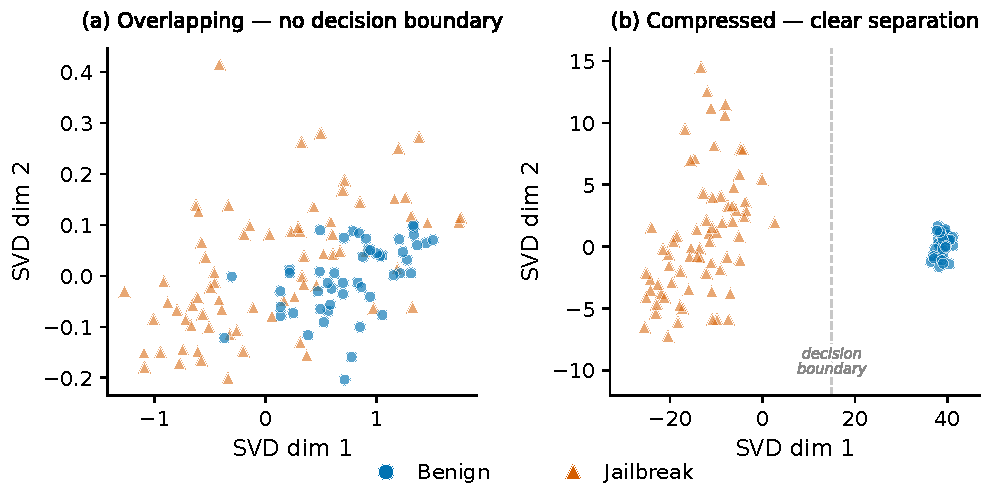
\includegraphics[width=\columnwidth]{figures/paper/fig4_svd_subspace.pdf}
\caption{Test representations projected onto top-2 SVD directions. 9-class DAPT produces clear cluster separation absent in vanilla.}
\label{fig:svd_subspace}
\end{figure}

\paragraph{Deployment implications.}
Our findings suggest a capacity-aware deployment strategy. At base scale (125--184M), any domain-relevant classification objective recovers OOD detection: scrambled labels perform equivalently on template attacks, so practitioners need not invest in annotation quality for this regime. When facing strategy-diverse attacks (e.g., ActorAttack), the label effect resurfaces ($d$\,=\,0.44), favoring semantically meaningful taxonomies. At sufficient capacity ($\geq$355M), DAPT becomes unnecessary and potentially counterproductive; the decision to adapt should be conditioned on encoder scale. Independent of adaptation choice, few-shot benign calibration (10--25 conversations per deployment domain) resolves false-positive rates without requiring target-domain attack data (calibration curves in Appendix~\ref{app:calibration}), enabling deployment across platforms with minimal data collection. The 184M-parameter pipeline maintains 24.3$\times$ inference speedup over LLM-as-judge alternatives (43$\times$ fewer parameters; Appendix~\ref{app:efficiency}), making it suitable for real-time monitoring at scale.

\section{Conclusion}

Classification DAPT recovers OOD detection at base scale (F1\,=\,0.97--1.0 vs.\ vanilla 0.26--0.31), though not under mixed-LLM training on diverse attacks (ActorAttack F1\,=\,0.504); on single-turn human-authored data, the hierarchy reverses (ToxicChat MLM 0.837 vs.\ classification 0.596), making these advantages condition-specific and counterproductive at 355M. Few-shot adaptation reduces FPR from 58--68\% to 0--1.5\%; this ablation framework provides a template for future controlled studies of domain adaptation in safety-critical natural language processing (NLP) tasks.

\section*{Limitations}
\label{sec:limitations}

\begin{itemize}[nosep,leftmargin=*]
\item \textbf{Synthetic data.} All findings derive from synthetic conversations (single LLM, Qwen3-8B; 350 training, 3 seeds); the hierarchy reverses on human single-turn data (ToxicChat), and no human-generated multi-turn jailbreak dataset exists.
\item \textbf{IID benign assumption.} OOD F1 assumes IID benign data; few-shot adaptation recovers performance but is validated on only two platforms ($n \leq 50$).
\item \textbf{Scope.} Only persuasion-mediated multi-turn attacks at base-to-large scale (125--355M); single-turn token-level attacks and non-text modalities are not addressed.
\end{itemize}

\section*{Ethical Considerations}

This work is defensive: it improves detection of multi-turn jailbreak attacks rather than developing new attacks. We acknowledge dual-use risk, as the persuasion taxonomy could inform adversarial actors. We mitigate this by using only synthetic conversations (no real harmful content), withholding attack-generation prompts, and focusing contributions on detection mechanisms. No human subjects were involved; all data will be released under CC BY-NC 4.0.
